\chapter{Teknologi}
\label{ch:technology}
Dette kapittelet redegjør kort for de ulike teknologiene som er relevante
for avstandsoppfølging i dette prosjektet: skyteknologi og skyløsninger, protokoller og metoder
for kommunikasjon, plattformer for elektronikkprototyping og sensorer og aktuatorer.

\section{Skyteknologi}
\blindtext

\subsection{Skybasert tingenes internett}
%Skkerhet, personvern, kvalitetsattributter

\subsection{AWS IoT}
Amazon sin \gls{iot}-løsning i skyen (\gls{aws} \gls{iot}) ble annonsert 9. oktober 2015.
Viktige aspekter av denne løsningen er AWS IoT Device SDKs som tilkobler mot 
en \textit{device gateway}, og en \textit{rules engine} som tillater løsningen å integrere
mot andre AWS-tjenester. Se figur \ref{fig:awsiot_how} for arkitekturoversikt.
Denne arkitekturen likner veldig på den \citet{iot_harvard_smart} foreslo i kapittel \ref{ch:background}.

\textit{Thing registry} er en liste av alle enheter tilkoblet tjenesten, og en \textit{device shadow}
holder styr på tilstanden til en enhet som kan hentes eller modifiseres fra andre applikasjoner.

\begin{figure}
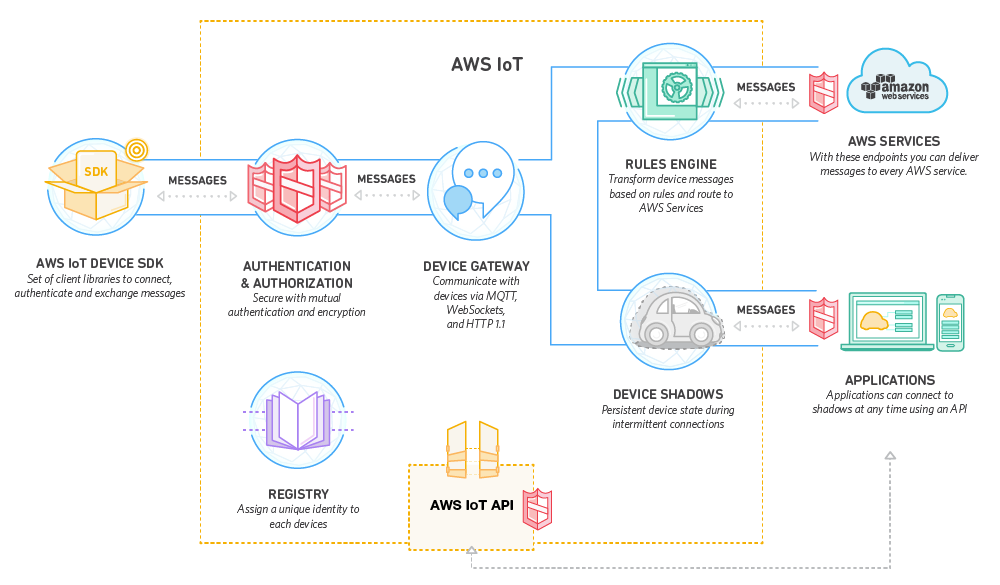
\includegraphics[width=1.0\textwidth,center]{fig/awsiot_how}
\caption{AWS IoT: Hvordan det virker \citep{aws_works}}
\label{fig:awsiot_how}
\end{figure}

\subsubsection{AWS IoT Device SDKs}
SDK-er er åpen kildekode på Github, og er tilgjengelige for embedded C, JavaScript (Node.js og nettleser),
Arduino Yún, Java, Python, iOS og Android \citep{aws_sdks}.

\subsubsection{Sikkerhet: Autentisering og tilgangskontroll}
AWS IoT tilbyr ende-til-ende-kryptering og gjensidig autentisering av alle meldinger med
\gls{tls} og klientside-X.509-sertifikater. Andre autentiseringsmetoder som Amazon sin egen SigV4-protokoll
er tilgjengelig også.

\subsubsection{Device gateway}
\textit{Device gateway} fungerer som en skalerbar meldingsbroker basert på publish-subscribe-mønsteret,
med støtte for MQTT (publish/subscribe), MQTT over WebSockets (publish/subscribe) og HTTP (publish).

\subsubsection{Rules engine}
Regelmotoren evaluerer innkommende meldinger etter at de passerer igjennom en \textit{device gateway},
og videresender disse meldingene til resten av AWS-økosystemet avhengig av hvilke regler som er satt opp.
Dette betyr at meldinger for eksempel kan bli endret og sendt videre, lagret i en database, aggregert i en
dataanalyseløsning og brakt videre til andre skytjenester. \citet{aws_works} nevner AWS Lambda, Amazon Kinesis,
Amazon S3, Amazon Machine Learning, Amazon DynamoDB, Amazon CloudWatch og Amazon Elasticsearch Service som mulige
integrasjoner.

\subsubsection{Device shadows}
Alle enheter koblet til \textit{device gateway} har en \textit{thing shadow} som er et JSON-dokument
med nåværende tilstand og informasjon om enheten. En \textit{thing shadow} til en ting er alltid tilgjengelig,
selv om enheten er koblet fra Internett. Den kan alltid bli hentet og endret over HTTP eller MQTT. En \textit{thing shadow}
er identifisert med sitt unike navn. AWS IoT reserverer emnenavnene \textit{get}, \textit{update}
og \textit{delete} for å kommunisere med \textit{device shadows}.

\subsubsection{Thing registry}
Et \textit{thing registry} er en JSON-liste av alle tingene som er tilkoblet til tjenesten. Hver ting
har et navn, og kan valgfritt ha attributter i nøkkel-verdi-par, for eksempel modellnavn og watt
for en lyspære. Det er mulig å lage forskjellige typer ting og assosierere disse typene med en ting.

\subsection{Microsoft Azure IoT Hub}
Microsoft Azure IoT Hub har mange av de samme egenskapene som AWS IoT med andre navn: \textit{cloud gateway},
\textit{device twins} og \textit{identity registry}. Autentisering gjøres enten med et unikt token per enhet eller med
X.509-sertifikater. I praksis spiller det nok ikke så stor rolle hvilken av disse skytjeneste man velger. 

\begin{figure}
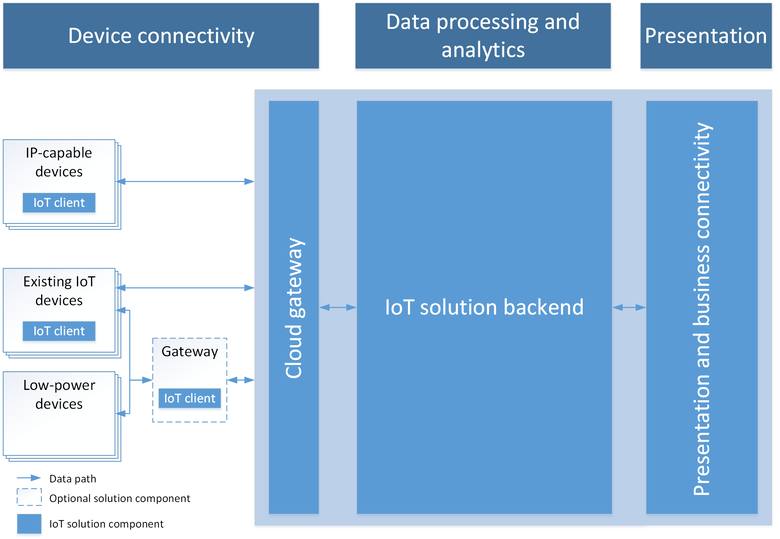
\includegraphics[width=1.0\textwidth,center]{fig/iot-reference-architecture}
\caption{Microsoft Azure IoT Hub: Løsningsarkitektur} % @Todo: Sitering?
\label{fig:azure_iot}
\end{figure}

% \section{Utviklingsmiljø} @ TODO: Skal dette være med egentlig? Er det relevant å bable om Node.js her?

\section{Protokoller og kommunikasjon}
\blindtext

\subsection{Bluetooth Low Energy}
\gls{ble}, tidligere markedsført som Bluetooth Smart, ble en del av Bluetooth-standarden fra versjon 4. BLE er egnet
for trådløs direktekommunikasjon mellom små enheter med lavt strømforbruk.

Bluetooth-standarden opererer med applikasjonsprofiler som beskriver hvordan man skal samhandle med
en Bluetooth-enhet. Profilene er bygget på generic attribute profile (GATT), en spesifikasjon for å sende og motta
små databiter (attributter) over en datalink. % @TODO: Kilde? https://www.bluetooth.com/specifications/generic-attributes-overview
En profil har typisk flere ulike tjenester, som igjen har flere ulike karakteristikker (se figur \ref{fig:gatt}).
Karakteristikkene har ulike egenskaper, attributtverdi og en databeskriver. Egenskapene definerer hvilke operasjoner som er lov
til å gjøre på en attributtverdi, for eksempel lese, skrive og lytte på. Bluetooth-standarden definerer en rekke standardiserte
profiler på \url{bluetooth.com}, blant annet \textit{Pulse Oximeter Service} og \textit{Battery Profile}.

\begin{figure}
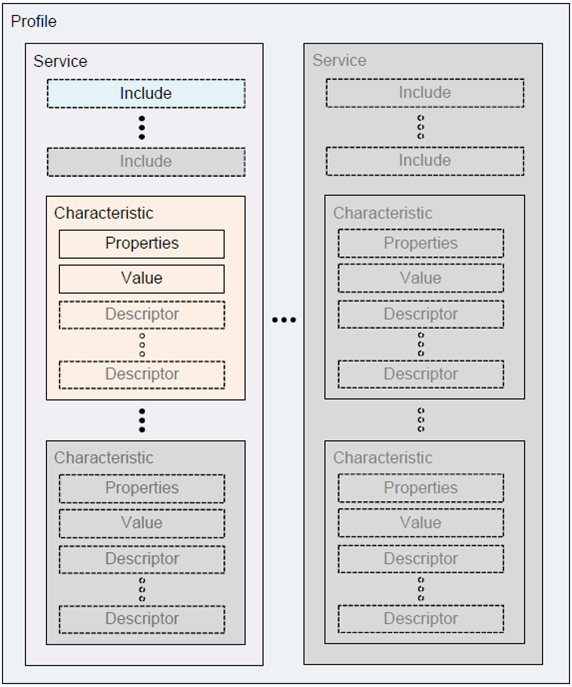
\includegraphics[width=0.6\textwidth,center]{fig/gatt}
\caption{Hierarki for GATT-profiler} % @TODO: Kilde? https://www.bluetooth.com/specifications/generic-attributes-overview
\label{fig:gatt}
\end{figure}

\subsubsection{Sikkerhet i BLE}
De største sikkerhetsproblemene til BLE generelt er passiv tyvlytting, «man-in-the-middle»-angrep (MITM) og identitetssporing.
Bluetooth 4.0 ble annonsert i 2010, og er nå delvis utdatert når det gjelder sikkerhet. Alle paringsmetodene
til 4.0 og 4.1 kalles for \textit{LE Legacy Pairing}. 

For å unngå passiv tyvlytting, krypterer BLE dataen som sendes mellom to enheter med en sikker blokkchiffer (AES-CCM). Problemet oppstår
i nøkkelutvekslingen mellom de to enhetene. I den vanligste paringsmetoden i \textit{LE Legacy Pairing}, Just Works\texttrademark,
brukes en svak midlertidig nøkkel (nøkkelen er tallet 0). Dermed er det enkelt for en angriper å finne ut hva korttidsnøkkelen
blir med rå datakraft og gjetting. Andre paringsmetoder eksisterer, men disse trenger brukerinteraksjon eller andre trådløse protokoller (NFC).
De er imidlertid rimelig sikre mot MITM.
% @TODO: kilde: https://eewiki.net/display/Wireless/A+Basic+Introduction+to+BLE+Security

4.2 introduserer \textit{LE Secure Connections}. I denne utgaven av Just Works\texttrademark-paring blir det kun generert
én langtidsnøkkel ved hjelp av «Elliptic Curve Diffie Hellman» (ECDH) asymmetrisk kryptering. Dette løser problemet med passiv
tyvlytting, men forbindelsen er fortsatt sårbar for MITM siden autentisering mangler. Et lite tillegg til Just Works\texttrademark
der man sammenligner om to verdier er like gjør denne metoden sikker mot MITM.

Etter at enhetene er paret, er det mulig å lagre nøklene på hver enhet slik at de kan gjenbrukes uten å gå igjennom hele
paringsprosessen på nytt. Dette kalles bonding.

Bluetooth 5 som lanseres våren 2017 lover lengre rekkevidde, økt hastighet 

%https://electronics.stackexchange.com/questions/284056/can-ble-transactions-be-encrypted-without-pairing
%https://security.stackexchange.com/questions/100554/is-bluetooth-4-0-traffic-encrypted-by-default-design
%https://piratecomm.wordpress.com/2014/01/19/ble-pairing-vs-bonding/
%https://community.nxp.com/thread/332191
\blindtext

\subsection{WebSockets og MQTT}
WebSockets er en protokoll for applikasjonslaget på toppen av \gls{tcp}
som gjør det mulig med toveiskommunikasjon gjennom en enkelt \gls{tcp}-socket.
I følge \citet{rfc6455} ble protokollen introdusert for å unngå tungvint \gls{http}-polling.

Websockets har et lite klient-\gls{api} der en kan få en god oversikt ved å lese
kodesnutt \ref{lst:websockets}. \gls{api}-et er basert på eventer, og forskjellige callback-funksjoner
vil bli kalt når det skjer noe spesielt, for eksempel når en ny melding er sendt til klienten eller
når tilkoblingen lukkes. Protokollen støtter \gls{tls}, og er implementert i alle de største nettleserne.
Den kan også brukes i andre miljøer og språk med gode nettverksbyggeklosser.

\begin{minipage}{\linewidth}
\begin{lstlisting}[frame=single, language=JavaScript,
    caption=WebSockets: JavaScript-eksempelkode, label=lst:websockets]
    //Initiate a new secure WebSocket connection with TLS
    const ws = new WebSocket("wss://address:port");

    //Attach functions to event handlers
    ws.onmessage = function(e) {
        var data = JSON.parse(e.data);
    };

    ws.onclose = function() {} //connection is closed

    ws.onerror = function() {} //something went wrong
    
    ws.onopen = function() {
        ws.send(JSON.stringify({ msg: "Hello, World" }));
    }
\end{lstlisting}
\end{minipage}

\gls{mqtt} er et lettvekt og meldingbasert klient-tjener-protokoll bygget for \gls{iot}-kommunikasjon
og \gls{m2m} \citep{mqtt_standard}. Den er designet for å bruke lite data og fungere bra på
dårlige nettverksforbindelser. \gls{mqtt} kjører direkte på \gls{tcp}/IP eller over WebSockets.

Protokollen er basert på «publish-subscribe»-meldingsmønsteret. En klient kan publisere hva som helst til
et \textit{emne (topic)} (streng, eller liste av strenger). En annen klient som abonnerer på det samme emne
vil motta datapakken fra den andre klienten. Dette gir de følgende klientmetodesignaturene for \gls{mqtt}:

\begin{verbatim}
    connect(mqtt://address:port)
    subscribe(topic: String | list of topics: String)
    unsubscribe(topic: String | list of topics: String)
    publish(topic: String, payload: String/binary)
    onMessageReceived(topic: String, payload: String/binary)
    close()
\end{verbatim}

\gls{mqtt}-brokeren tar i mot og behandler innkommende klienttilkoblinger og stopp av abonnement. I tillegg
mottar den meldinger og sender meldinger videre til klienter som abonnerer på et emne.

\subsection{UART og GPIO}
\blindtext

\section{Prototypeplattformer}
\blindtext
\subsection{Raspberry Pi}
\blindtext
\subsection{Arduino}
\blindtext
\subsection{Tessel}
\blindtext

\section{Sensorer og aktuatorer}
\blindtext
\subsection{Pulsoksimeter}
%https://www.protocentral.com/sensors/1030-protocentral-pulse-oximeter-heart-rate-sensor-based-on-max30100.html
\blindtext
\subsection{Fingeravtrykk}
\blindtext
\subsection{Trykknapp}
\blindtext
\subsection{RGB LED}
\blindtext
